%%%%%%%% this is the data section
% \documentclass[12pt, amstex, letterpaper] {report} %{article}


\usepackage[margin=1in]{geometry}
\topmargin -0.5in \textwidth 6.5in \textheight 9in
\footskip .5in
\headheight 0.3in


\usepackage{Sweave}

\DefineVerbatimEnvironment{Sinput}{Verbatim} {xleftmargin=0em,frame=single}
\DefineVerbatimEnvironment{Soutput}{Verbatim} {xleftmargin=0em,frame=single}

\usepackage{amssymb, mathrsfs, amsmath, amsfonts}
\usepackage{enumerate, comment}
\usepackage{hyperref, natbib,apalike, float} %cite
\usepackage{color, multirow, setspace, fancyhdr,graphicx}
\usepackage{undertilde}
\usepackage[bottom]{footmisc}
\usepackage{graphicx}
\usepackage{framed}
\usepackage{subcaption}
\usepackage{amsthm}

%\doublespacing
\pagestyle{empty}
\pagestyle{fancy}
\lhead{ }
%\rhead{May 2016}
\fancyfoot{ }
\rfoot{Dissertation $|$ \thepage}
\lfoot{Chris Vanlangenberg}
\date{}

\includecomment{comment}

\newtheorem{theorem}{Theorem}[section]
\newtheorem{defn}{Definition}[section]
\newtheorem{prop}{Proposition}
\newcommand{\pro}[1]{\begin{prop}{#1}\end{prop}}

%\newtheorem{proof}{proof}
\newtheorem{rmk}{Remark}
\newcommand{\rmark}[1]{\begin{rmk}{#1}\end{rmk}}

\numberwithin{equation}{section}
\renewcommand{\footrulewidth}{0.1pt}
\renewcommand{\headrulewidth}{0.1pt}


\newcommand{\eqn}[1]{\begin{equation}{#1}\end{equation}}

\newcommand{\beq}{\begin{equation}}
\newcommand{\eeq}{\end{equation}}
%\renewcommand\refname{Literature}
\newcommand{\blue}[1]{\textcolor{blue}{\emph{#1}}}
\newcommand{\red}[1]{\textcolor{red}{\emph{#1}}}
\newcommand{\twoc}[2]{{\textcolor{blue}{#1}} and {\textcolor{red}{#2}}}


\newcommand{\xn}{x_1,\ldots, x_n}
\newcommand{\Xn}{X_1,\ldots, X_n}
\newcommand\floor[1]{\lfloor{#1}\rfloor}
\newcommand\ceil[1]{\lceil{#1}\rceil}

\newcommand{\X}{\mathcal{X}}
\newcommand{\Sp}{\mathbb{S}}
\newcommand{\R}{\mathbb{R}}
\newcommand{\C}{\mathbb{C}}
\newcommand{\pd}{positive definite }



\newcommand{\code}[1]{{\small\texttt{#1}}}
\newcommand{\pkg}[1]{{\normalfont\textsf{#1}}}
\newcommand{\var}[1] {{\normalfont\textbf{#1}}}
\newcommand{\Cm}{$C_m(\phi_P, \phi_Q)\ $}

\newcommand{\jun}{\cite{JunStein2008}}
% \begin{document}
% \section{Simulations}

What does it mean by spatial data? In general, spatial data or in other words geospatial data is information about a physical object or a measurement that can be represented by numerical values in a geographic coordinate system. As \cite{Cressie1993} pointed out spatial data appeared to be in the form of maps in 1686 and spatial modeling paper in 1907. There are many questions that geoscientists and engineers are interested about spatial data. Many questions naturally arise such as how to model a spatial process and then use the model to make predictions about unobserved locations. There are many challenges when modeling spatial data; every point (location observed) is a random variable and only one observation/measurement is available. However, the number of unknowns to estimate are quite large compared to the available data, which is definitely a high-dimensional problem. As an example, if data were observed at 10 locations, one is estimating the variance-covariance matrix to characterize the spatial dependency for future predictions. Then there will have 55 unknown entities in the variance-covariance matrix to be estimated.

\begin{figure}[H]
\label{MSU_data_latitude}
\centering
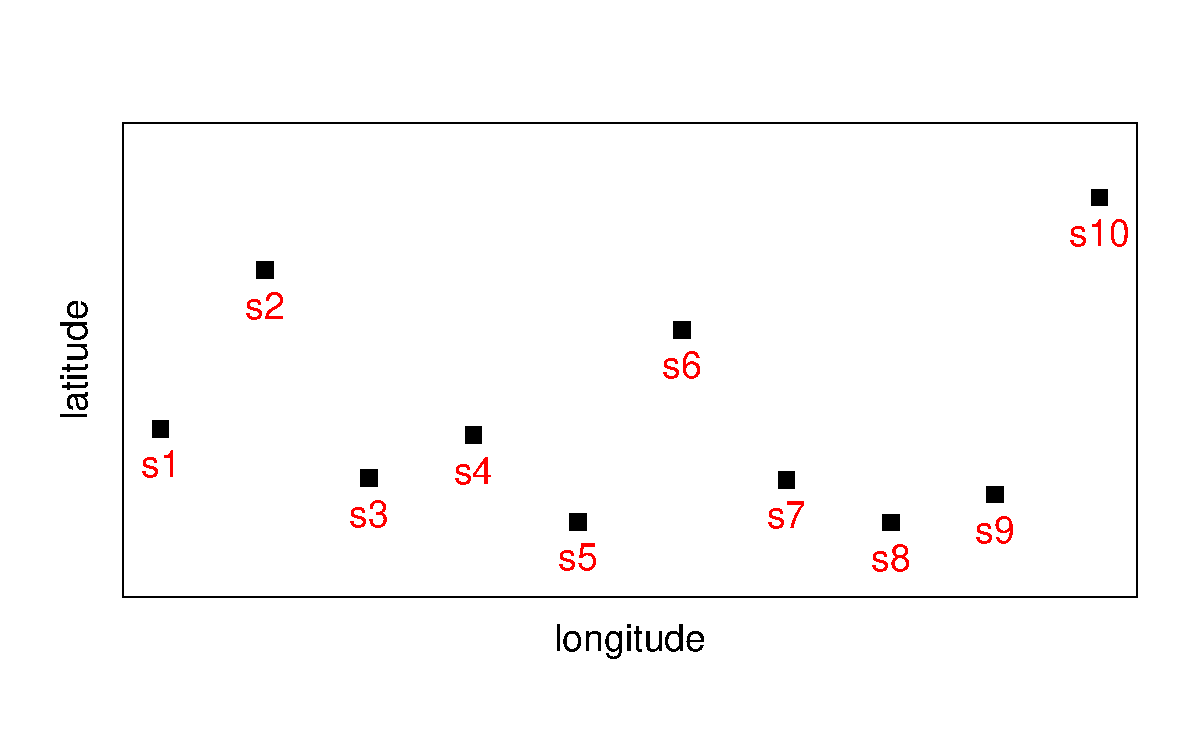
\includegraphics [height=4in, keepaspectratio]{location.pdf}
\caption{Some arbitary saptial data at 10 random locations}
\end{figure}

\newpage
\subsection{MSU data}

Since 1978 Microwave Sounding Units (MSU) measure radiation emitted by the earth's atmosphere from NOAA polar orbiting satellites. The different channels of the MSU measure different frequencies of radiation proportional to the temperature of broad vertical layers of the atmosphere. Tropospheric and lower stratospheric temperature data are collected by NOAA's TIROS-N polar-orbiting satellites and adjusted for time-dependent biases by the Global Hydrology and Climate Center at the University of Alabama in Huntsville (UAH)\footnote{\url{https://www.ncdc.noaa.gov/temp-and-precip/msu/overview}}. More information about how the data is been processed can be found in \cite{ChristySpencerBraswell2000}. Satellites do not measure temperature directly but measure radiances in various wavelength bands and then mathematically inverted to obtain the actual temperature.

% Channel 2 mainly measures tropospheric temperatures, while Channel 4 measures temperatures in the lower stratosphere. The analysis of the satellite temperature record represented here begins in 1979.

\begin{figure}[H]
\label{MSU_data}
\centering
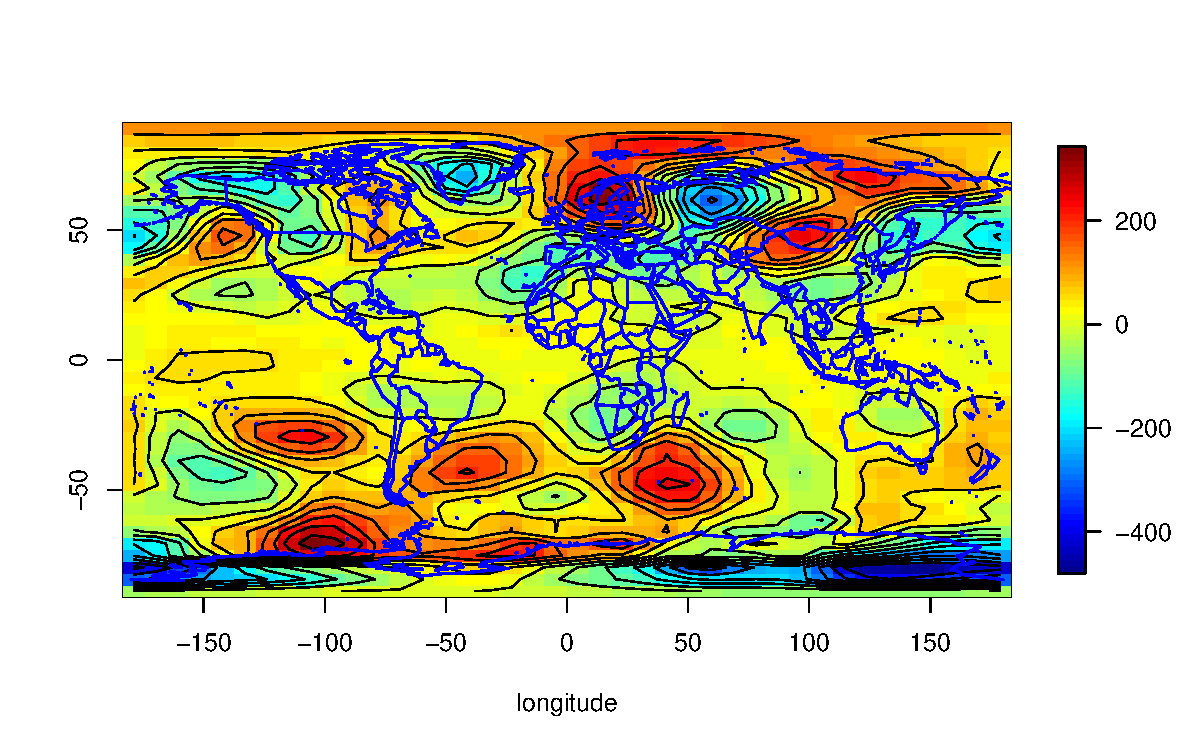
\includegraphics [height=5in, keepaspectratio]{MSU_data.pdf}
\caption{MSU data observed (without removing any spatial trends) in August 2002 : resolution $2.5^\circ \mbox{ latitude} \times 2.5^\circ \mbox{ longitude}$. It is easy to observe that variation is higher towards the north and south poles.}
\end{figure}

The MSU data were observed at $2.5^\circ \mbox{latitude} \times 2.5^\circ \mbox{longitude}$ with total number of data observations of size 10368.


% \begin{figure}[H]
% \label{MSU_data_contour}
% \centering
% 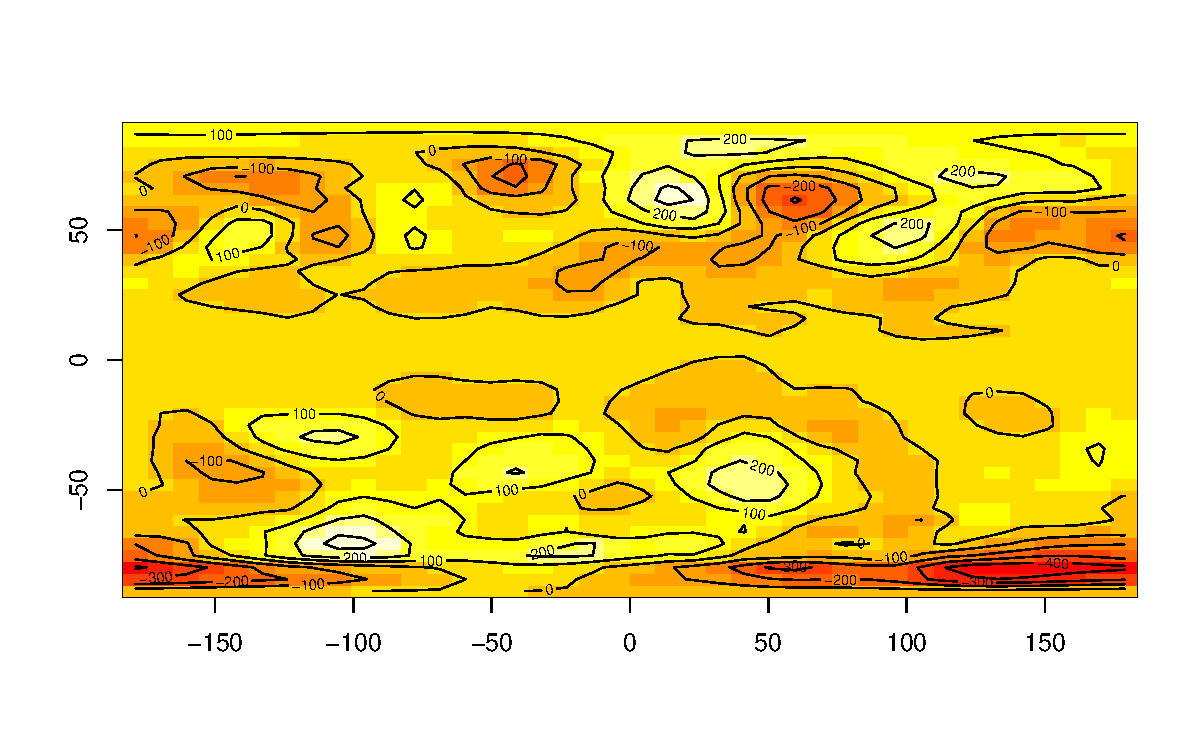
\includegraphics [height=4in, keepaspectratio]{MSU_data_contour.pdf}
% \caption{August 2002, MSU data contour plot : resolution $2.5^0 latitude \times 2.5^0 longitude$}
% \end{figure}

\begin{figure}[H]
\label{MSU_data_latitude}
\centering
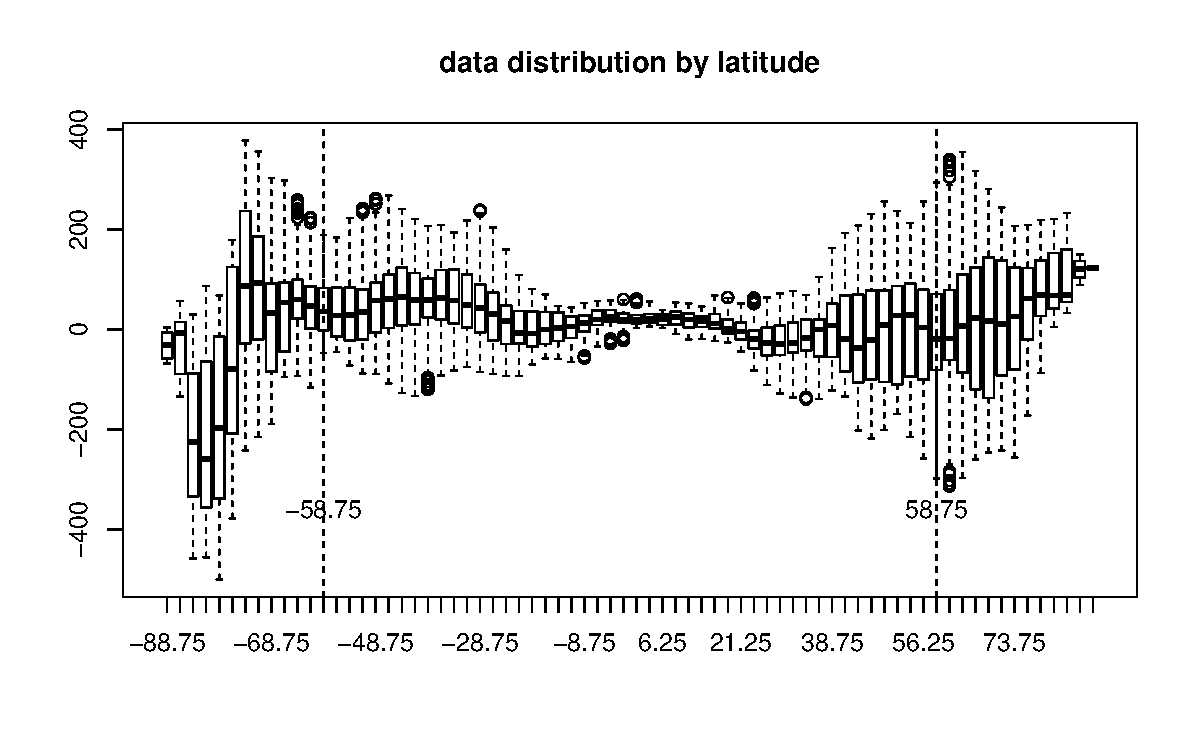
\includegraphics [height=5in, keepaspectratio]{MSU_data_latitude.pdf}
\caption{MSU data (August 2002), data distribution at each latitude (the spread is very high near north and south poles)}
\end{figure}

\begin{figure}[H]
\centering
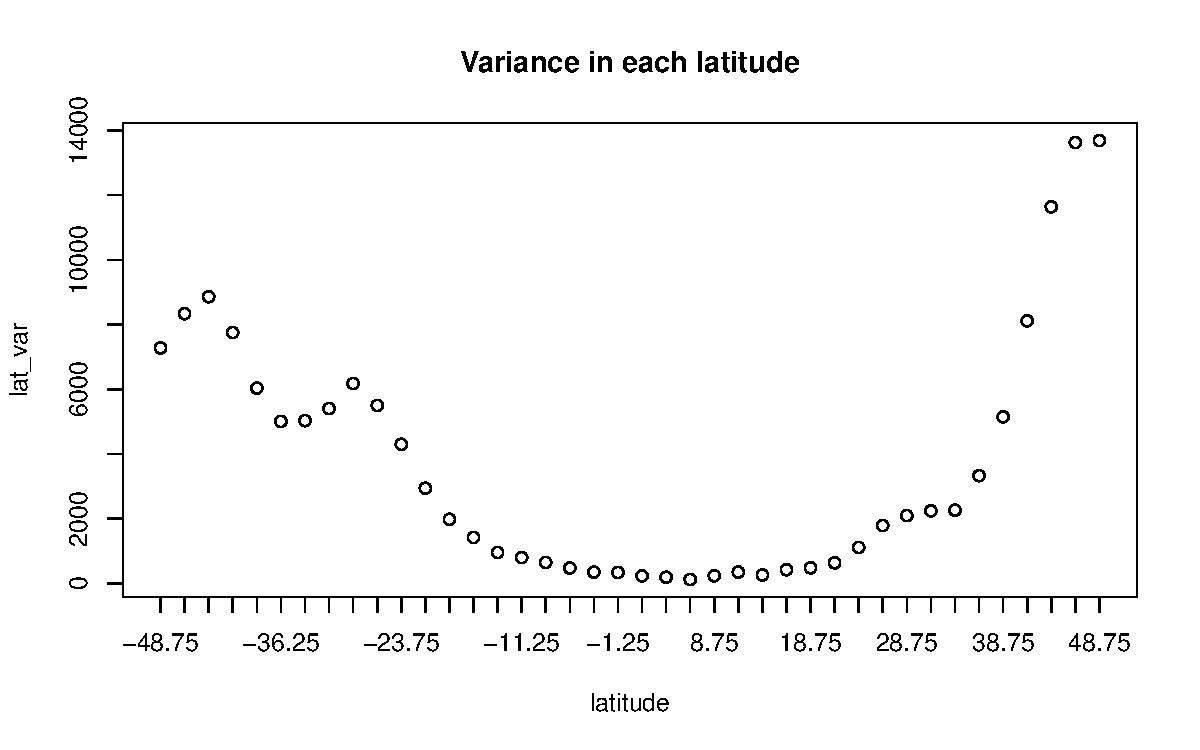
\includegraphics [height=5in, keepaspectratio]{MSU_data_var_lat.pdf}
\caption{MSU data (August 2002) between $60^\circ S$ and $60^\circ N$, the variance at each latitude (variance is almost zero near the equator)}
\label{MSU_data_var_lat}
\end{figure}

\newpage
\subsection{TOMS data}

Extracted from \cite{Stein2007} ``The Nimbus-7 satellite carried a Total Ozone Mapping Spectrometer (TOMS) instrument that measured total column ozone daily from November 1, 1978 to May 6, 1993. This satellite followed a Sun-synchronous polar orbit with an orbital frequency of 13.825 orbits a day (cycle time about 104 minutes). As the satellite orbited, a scanning mirror repeatedly scanned across a track about 3000 km wide, each track yielding 35 total column ozone measurements. This version of the data is known as Level 2 and is publicly available \footnote{\url{http://disc.sci.gsfc.nasa.gov/data/datapool/TOMS/Level 2/}}. "

\begin{figure}[H]
\label{TOMS_data}
\centering
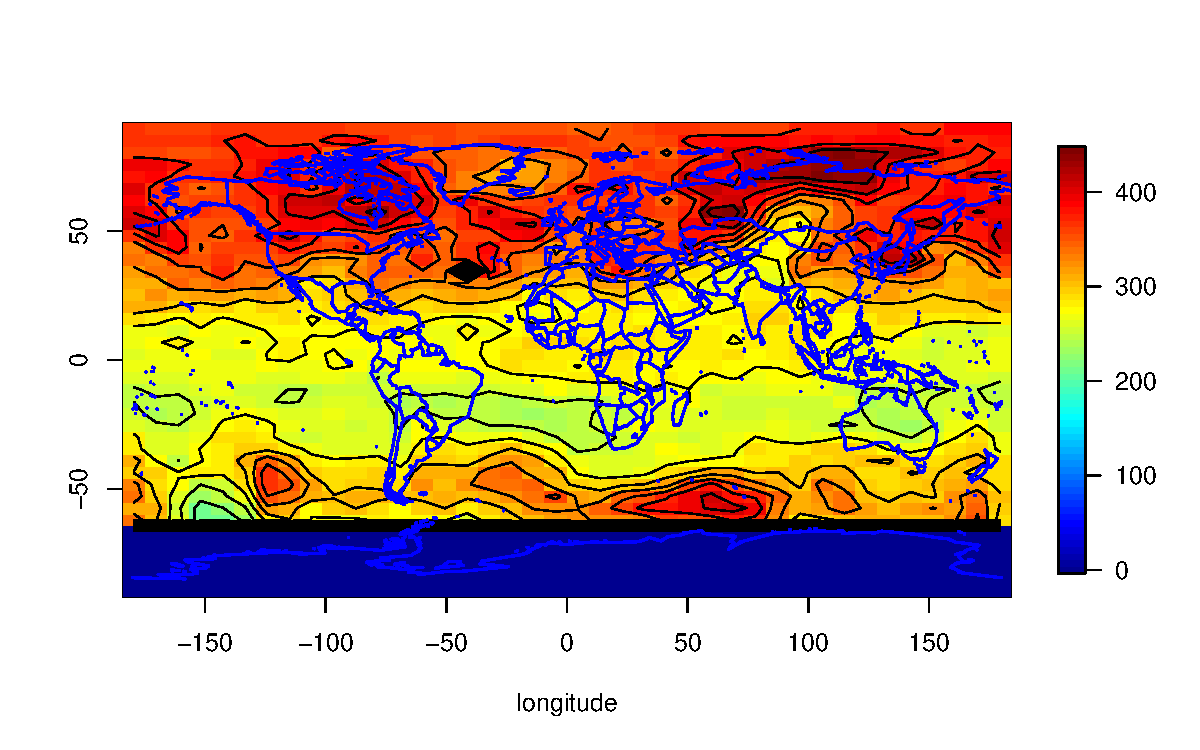
\includegraphics [height=5in, keepaspectratio]{TOMS_data.pdf}
\caption{TOMS data: resolution $1^\circ \mbox{latitude } \times 1.25^\circ \mbox{ longitude}$ in May, 1-6 1990. The instrument used backscattered sunlight, therefore measurements were not available south of $73^\circ S$ during this week.}
\end{figure}

There were some missing values in this data set. \cite{Stein2007} used the average of 8 neighboring locations to replace the missing values. Further, he used spherical harmonics with associated Legendre polynomials of up to 78 covariates to remove the spatial trends to study axial symmetry of the data.
\begin{figure}[H]
\centering
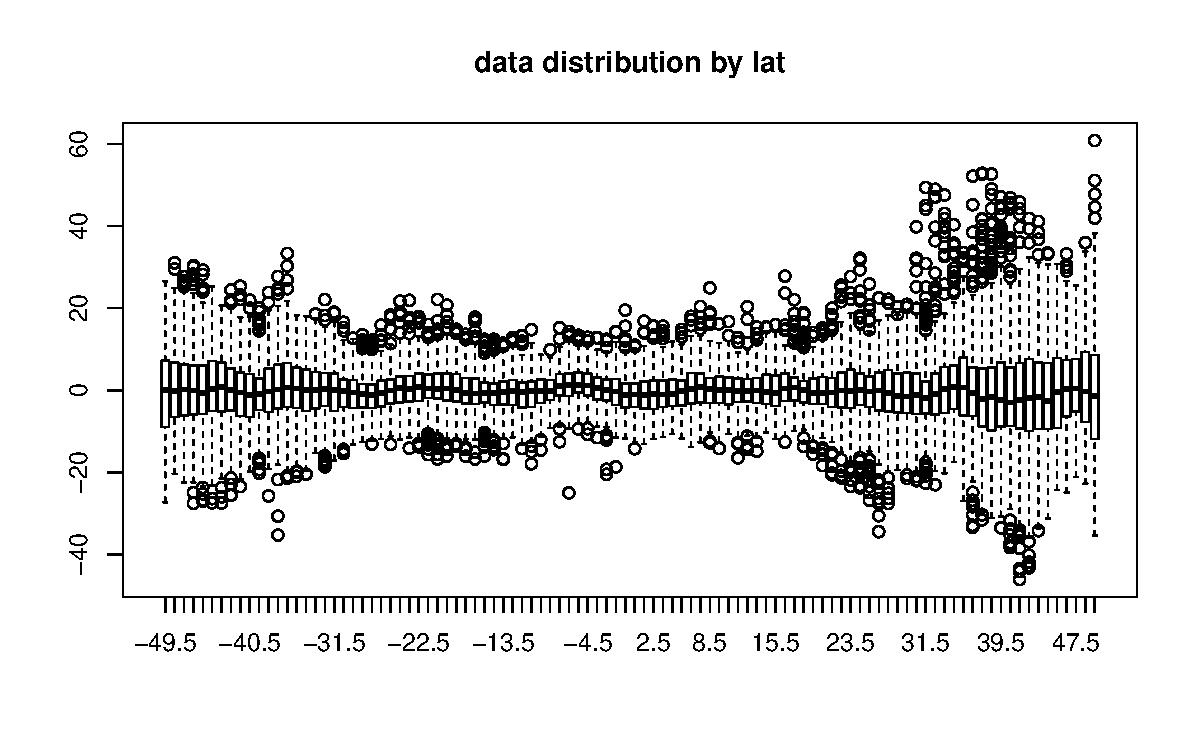
\includegraphics [height=5in, keepaspectratio]{TOMS_data_latitude.pdf}
\caption{TOMS data: data distribution at each latitude (data between $50^\circ S$ and $50^\circ N$ were considered)}
\label{TOMS_data_latitude}
\end{figure}

\begin{figure}[H]
\centering
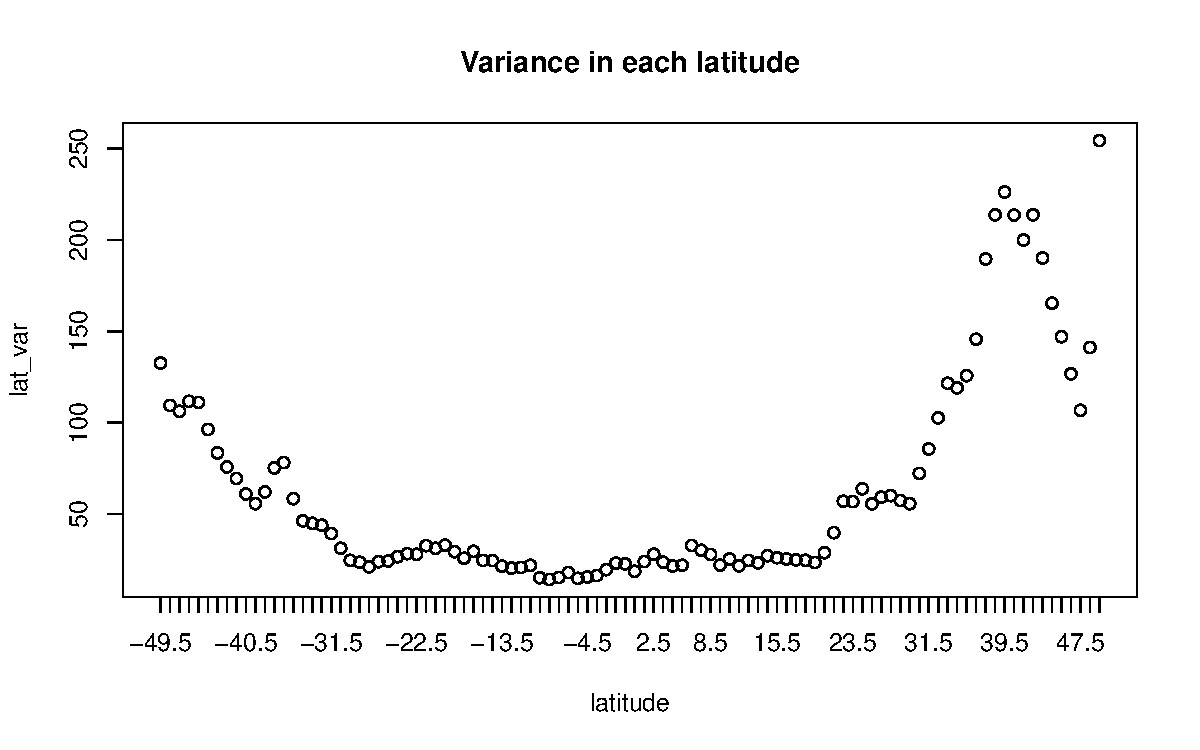
\includegraphics [height=5in, keepaspectratio]{TOMS_data_var_lat.pdf}
\caption{TOMS data: between $50^\circ S$ and $50^\circ N$, the variance at each latitude (variance is almost zero near the equator)}
\label{TOMS_data_var_lat}
\end{figure}

\newpage
\subsection{Challenges}

\begin{enumerate}
\item There have been extensive statistical research on methodologies and techniques developed under the Euclidean space $R^d$. These approaches that are valid in $R^d$ have been applied to analyze global-scale data in recent years, due to global networks and satellite sensors that have been used to monitor a wide array of global-scale processes and variables. However, this can have unforeseen impacts, such as making use of models that are valid in $R^d$ but in fact might not be valid under spherical coordinate systems. \cite{HuangZhangRobeson2011} have investigated some of commonly used covariance models that are valid in $R^d$, and they pointed out that many of those are actually invalid on the sphere.
\item Note that, as we will see later, the spectral representation of the process on the sphere is a summation of Legendre polynomials, which is distinct from its planar counterpart as represented by an integration of Bessel functions. This distinction can be understood through group representation theory, which is the basis for an exciting new line of research we are currently pursuing.
\end{enumerate}


%\blue{if more time will add further information, we will use the trend free data}
%\end{document} 